\documentclass{article}%
\usepackage[T1]{fontenc}%
\usepackage[utf8]{inputenc}%
\usepackage{lmodern}%
\usepackage{textcomp}%
\usepackage{lastpage}%
\usepackage{parskip}%
\usepackage[top=1.2in,bottom=1in,left=0.6in,right=0.6in,headsep=0.8in]{geometry}%
\usepackage{amsmath}%
\usepackage{graphicx}%
\usepackage{needspace}%
\usepackage{color}%
\usepackage{longtable}%
\usepackage{multirow}%
\usepackage[table]{xcolor}%
\usepackage{fancyhdr}%
\usepackage{tabularx}%
%
\definecolor{OsdagGreen}{HTML}{D5DF93}%
\fancypagestyle{header}{ 
\renewcommand{\headrulewidth}{0pt}%
\renewcommand{\footrulewidth}{0pt}%
\fancyhead{ 
}%
\fancyfoot{ 
}%
\fancyhead[C]{ 
\begin{tabularx}{\textwidth}{|l|p{6cm}|l|X|}%
\hline%
\rowcolor{OsdagGreen}%
Company Name&&Project Title&\\%
\hline%
\rowcolor{OsdagGreen}%
Group/Team Name&&Subtitle&\\%
\hline%
\rowcolor{OsdagGreen}%
Designer&&Job Number&\\%
\hline%
\rowcolor{OsdagGreen}%
Date&20 /05 /2020&Client&\\%
\hline%
\end{tabularx}
}%
\fancyfoot[R]{ 
Page \thepage\ of \pageref{LastPage}
}
}%
%
\begin{document}%
\normalsize%
\pagestyle{header}%
\section{Input Parameters}%
\label{sec:InputParameters}%
\renewcommand{\arraystretch}{1.2}%
\begin{longtable}{|p{5cm}|p{2cm}|p{2cm}|p{2cm}|p{5cm}|}%
\hline%
\hline%
\multicolumn{3}{|c|}{Module}&\multicolumn{2}{|c|}{Tension Members Bolted Design}\\%
\hline%
\hline%
\multicolumn{3}{|c|}{Axial (kN) *}&\multicolumn{2}{|c|}{1000.0}\\%
\hline%
\hline%
\multicolumn{3}{|c|}{Length(mm) *}&\multicolumn{2}{|c|}{18000.0}\\%
\hline%
\hline%
\multicolumn{3}{|c|}{Section Size*}&\multicolumn{2}{|c|}{Ref List of Input Section}\\%
\hline%
\hline%
\multicolumn{5}{|c|}{\textbf{Bolt Details}}\\%
\hline%
\hline%
\multicolumn{3}{|c|}{Diameter (mm)*}&\multicolumn{2}{|c|}{{[}30.0, 36.0{]}}\\%
\hline%
\hline%
\multicolumn{3}{|c|}{Grade *}&\multicolumn{2}{|c|}{{[}3.6, 4.6, 4.8, 5.6, 5.8, 6.8, 8.8, 9.8, 10.9, 12.9{]}}\\%
\hline%
\hline%
\multicolumn{3}{|c|}{Type *}&\multicolumn{2}{|c|}{Bearing Bolt}\\%
\hline%
\hline%
\multicolumn{3}{|c|}{Bolt hole type}&\multicolumn{2}{|c|}{Standard}\\%
\hline%
\hline%
\multicolumn{3}{|c|}{Bolt Ultimate Strength (N/mm2)}&\multicolumn{2}{|c|}{0.0}\\%
\hline%
\hline%
\multicolumn{3}{|c|}{Bolt Yield Strength (N/mm2)}&\multicolumn{2}{|c|}{0.0}\\%
\hline%
\hline%
\multicolumn{3}{|c|}{Slip factor (µ\_f)}&\multicolumn{2}{|c|}{0.3}\\%
\hline%
\hline%
\multicolumn{3}{|c|}{Type of edges}&\multicolumn{2}{|c|}{a {-} Sheared or hand flame cut}\\%
\hline%
\hline%
\multicolumn{3}{|c|}{Gap between beam and <br>support (mm)}&\multicolumn{2}{|c|}{0.0}\\%
\hline%
\hline%
\multicolumn{3}{|c|}{Are the members exposed to <br>corrosive influences}&\multicolumn{2}{|c|}{False}\\%
\hline%
\hline%
\multicolumn{5}{|c|}{\textbf{Safety Factors {-} IS 800:2007 Table 5 (Clause 5.4.1) }}\\%
\hline%
\hline%
\multicolumn{3}{|c|}{Governed by Yielding}&\multicolumn{2}{|c|}{$\begin{aligned}\gamma_{m0}&=1.1\end{aligned}$}\\%
\hline%
\hline%
\multicolumn{3}{|c|}{Governed by Ultimate Stress}&\multicolumn{2}{|c|}{$\begin{aligned}\gamma_{m1}&=1.25\end{aligned}$}\\%
\hline%
\hline%
\multicolumn{3}{|c|}{Connection Bolts {-} Bearing Type}&\multicolumn{2}{|c|}{$\begin{aligned}\gamma_{mb}&=0.0\end{aligned}$}\\%
\hline%
\end{longtable}%
\subsection{List of Input Section}%
\label{subsec:ListofInputSection}%
\renewcommand{\arraystretch}{1.2}%
\begin{longtable}{|p{8cm}|p{8cm}|}%
\hline%
\multicolumn{1}{|c|}{Section Size*}&\multicolumn{1}{|c|}{{[}'MCP 100', 'MC 100', 'LC 100', 'JC 100', 'MCP 125', 'MC 125*', 'MC 125', 'LC(P) 125}\\%
\hline%
\hline%
\multicolumn{1}{|c|}{ }&\multicolumn{1}{|c|}{', 'LC 125', 'JC 125'{]}}\\%
\hline%
\end{longtable}

%
\Needspace{10\baselineskip}%
\newpage%
\section{Design Checks}%
\label{sec:DesignChecks}%
\subsection{Selected Member Data}%
\label{subsec:SelectedMemberData}%
\renewcommand{\arraystretch}{1.2}%
\begin{longtable}{|p{5cm}|p{2cm}|p{2cm}|p{2cm}|p{5cm}|}%
\hline%
\hline%
\multirow{14}{*}{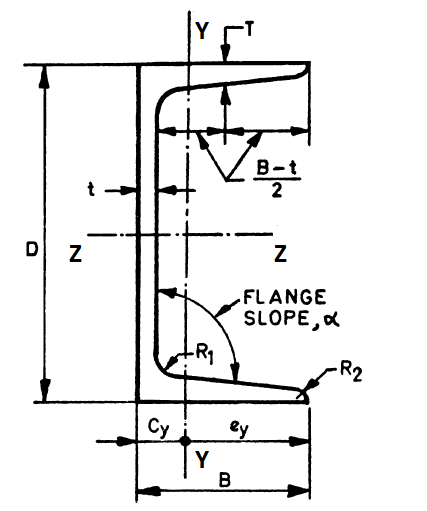
\includegraphics[width=5cm,height=5cm]{E:/workspace/Osdag3/ResourceFiles/images/Channel.png}}&\multicolumn{2}{|c|}{Section Size*}&\multicolumn{2}{|c|}{('MC 125*', 'Channels')}\\%
\cline{2%
-%
5}%
&\multicolumn{2}{|c|}{Material *}&\multicolumn{2}{|c|}{E 250 (Fe 410 W)A}\\%
\cline{2%
-%
5}%
&\multicolumn{2}{|c|}{Ultimate strength, fu (MPa)}&\multicolumn{2}{|c|}{410}\\%
\cline{2%
-%
5}%
&\multicolumn{2}{|c|}{Yield Strength , fy (MPa)}&\multicolumn{2}{|c|}{250}\\%
\cline{2%
-%
5}%
&Mass&13.7&Iz(mm4)&4340000.0\\%
\cline{2%
-%
5}%
&Area(mm2) {-} A&1750.0&Iy(mm4)&638000.0\\%
\cline{2%
-%
5}%
&D(mm)&125&rz(mm)&49.8\\%
\cline{2%
-%
5}%
&B(mm)&66&ry(mm)&19.1\\%
\cline{2%
-%
5}%
&t(mm)&6.0&Zz(mm3)&69500.0\\%
\cline{2%
-%
5}%
&T(mm)&8.1&Zy(mm3)&13600.0\\%
\cline{2%
-%
5}%
&FlangeSlope&96&Zpz(mm3)&0.0\\%
\cline{2%
-%
5}%
&R1(mm)&9.5&Zpy(mm3)&13600.0\\%
\cline{2%
-%
5}%
&R2(mm)&2.4&r(mm3)&19.1\\%
\cline{2%
-%
5}%
&Cy(mm)&19.2&&\\%
\cline{2%
-%
5}%
\hline%
\end{longtable}

%
\newpage%
\subsection{Spacing Checks}%
\label{subsec:SpacingChecks}%
\renewcommand{\arraystretch}{1.2}%
\begin{longtable}{|p{2.5cm}|p{7.5cm}|p{3cm}|p{3cm}|}%
\hline%
\rowcolor{OsdagGreen}%
Check&Required&Provided&Remarks\\%
\hline%
\endhead%
\hline%
Min.Diameter (mm)&&$\begin{aligned} d &=30.0\end{aligned}$&\\%
\hline%
Hole Diameter (mm)& &$\begin{aligned} d_0 &=33.0\end{aligned}$&\\%
\hline%
Min. Gauge (mm)&$\begin{aligned}p/g_{min}&= 2.5 ~ d&\\ =&2.5*30.0&=75.0\end{aligned}$&75&Row Limit (rl) = 2\\%
\hline%
Min. Edge Distance (mm)&$\begin{aligned}e/e`_{min} &=[1.5~or~ 1.7] * d_0\\ &=1.7*33.0=56.1 \end{aligned}$&60&\\%
\hline%
Spacing Check&$\begin{aligned} depth & = 2 * e + (rl -1) * g \\ & = 2 * 60+(2-1)*75 \\ & = 195\end{aligned}$&89.8&Fail\\%
\hline%
\end{longtable}

%
\newpage%
\subsection{Member Checks}%
\label{subsec:MemberChecks}%
\renewcommand{\arraystretch}{1.2}%
\begin{longtable}{|p{2.5cm}|p{4.5cm}|p{8cm}|p{1cm}|}%
\hline%
\rowcolor{OsdagGreen}%
Check&Required&Provided&Remarks\\%
\hline%
\endhead%
\hline%
Tension Yielding Capacity (kN)&1000.0&$\begin{aligned}T_{dg}~or~A_c&= \frac{1 * A_g ~ f_y}{\gamma_{m0}}\\ &= \frac{1*1750.0*250}{1.1}\\ &= 259.09\end{aligned}$&Fail\\%
\hline%
Slenderness&$\begin{aligned}\frac{K * L}{r} &\leq 400\end{aligned}$&$\begin{aligned}\frac{K * L}{r} &= \frac{1*18000.0}{19.1}\\ &= 942.41\end{aligned}$&Fail\\%
\hline%
\end{longtable}

%
\Needspace{10\baselineskip}%
\newpage%
\end{document}